\chapter{Сципион Африканский}


Привет. Сегодня я вам расскажу про настоящего "римского гуманиста" Публия Корнелия Сципиона Африканского. Этот человек воевал с Ганнибалом во Вторую Пуническую, победил его при Заме, а потом заключил с Карфагеном крайне щадящий мир. Ну, во всяком случае город не стёрли с лица земли и даже оставили пунийцам африканские владения. Вернувшись в Рим, Сципион и его сторонники набирают очень большой вес в политике, и поэтому последующие войны Рима тоже были крайне гуманны. В Греции Сципион не просто всё сжигает и завоёвывает, а освобождает греков от македонского ига, в результате чего те становятся "независимы", под римским протекторатом, естественно. А затем римляне отбивают агрессию Селевков против своих союзников, и наносят ему чудовищное поражение, но тоже проявляют гуманизм, и не добивают смертельно раненую Империю Селевкидов. А ограничиваются вытеснением её из Малой Азии и денежной контрибуцией. Воистину, Сципион Африканский и годы его правления были практически "Эпохой Просвещения" для римлян. С 205 г. до н.э., даты первого консульства после побед в Испании и до 184 г. до н.э., года, когда "партия войны" во главе с Катоном Старшим таки добила стареющего Сципиона. Два десятилетия Сципион Африканский и его окружение создавали очень интересную дипломатическую матрицу, которая, к сожалению, была не столь долговечной, но всё же довольно необычной по тем временам.


Во всяком случае так нам подаёт тему Тит Ливий, Полибий, да и общее мнение историографии примерно таково. Жили себе кровожадные сыны волчицы, жрали младенцев на завтрак и мочили всех, до кого могли дотянуться, без всякой жалости. Потом Сципион благодаря своим славным победам и общей крутизне попытался отучить латинов от "тотал крига" по любому поводу, вбить в них возможность мирного сосуществования с соседями и даже личным примером демонстрировал как можно и нужно вести дела. Войны гуманно выигрывал, создавал Республике имидж справедливой и умеренной в аппетитах державы. Но Рим хотел крови и не хотел слушать, поэтому, как только Сципион ослаб, латины отодвинули его сторонников от рычагов и занялись любимым делом — продолжили потрошить своих соседей без всякой жалости и гуманизма, совершать военные преступления и нести соседям войну и смерть.

А теперь давайте разбираться. Как мне кажется, попытки прилепить сюда моральные ярлыки и повесить всё на одного человека, это какая-то глупость. Причины всего вышеперечисленного, как обычно и бывает в истории, лежат на стыке географии и экономики, и очень косвенно определяются личностью, которая всё это дело воплощала на местности. У нас есть три последовательные войны, и у Рима были очень серьёзные причины в тот момент вести и закончить их именно так, как они закончились. То есть тут не Сципион кровожадных латинов уговаривал не убивать всех в тотал и приносить в жертву Марсу, а ему вполне чёткие инструкции из Рима приходили, общий смысл которых: "а резать мы их будем потом".

\section{Карфаген, Вторая Пуническая война.}

202 г. до н.э. Битва при Заме. Сципион наносит "Великому Пунийцу" его единственное за всю карьеру поражение, множит на ноль пунийскую армию и, казалось бы, сам Карфаген можно было брать голыми руками. Вместо этого Сципион заключает с пунами мир на очень скромных условиях. Разовая контрибуция, потеря всех заморских владений, потеря боевого флота и роспуск армии. Кроме того, сухопутные владения Карфагена частично уходят Нумидии, союзнице Рима. И... всё. Война окончена. При этом сам Карфаген и его богатейшие прибрежные города Рим не занимал и не грабил, оставил всё как есть. Зачем? Это было реально нетипично для войн того времени. Тут есть совершенно чёткая причина. У римлян прост всё хорошо было со здравым смыслом. Захватить Карфаген нереально, это мегаполис огромного масштаба, он всегда будет очагом сепаратизма. Включать же побеждённые народы в свой истеблишмент для Рима было неприемлемо. А просто сломать — нецелесообразно, регион прост придёт в запустение, и никакого профита с этого не будет. Поэтому его оставили как дойную корову, как и любой другой сделал бы на месте Рима. Разоружив, отрезав всё, что отрезается, но оставили. Торговля — это ведь логистика, развитие регионов, в неё вовлечённых, проникновение чуждой культуры, торговые связи с другими регионами. Убей торговлю — крупная держава атомизируется и начнёт стагнировать. Обратите внимание, с кем торговал Карфаген. Если за ними осталась только Африка, с условно независимыми кочевниками, а все прибрежные регионы западнее Греции контролировались Римом либо напрямую, либо косвенно. Западное Средиземноморье всегда было отсталым, относительно Востока. А сами римляне в торговлю не умели вообще. Убей Карфаген и всё, держава встанет в развитии благополучно. Там количество золота мало что решало само по себе, Карфаген оставляли как крупнейший в регионе транспортный и торговый узел, а также культурный и ремесленный центр. При этом пунам выдрали все зубы и зорко следили чтобы он не отращивал новые, причём как сами, так и с помощью нумидийцев. И заставили работать на Республику, чем успешно и пользовались потом долгие полвека. Рим навязывал Карфагену условия, по которым он мог с ним торговать, и были они далеко не равные. Как известно, лучший способ заключить хорошую сделку – это подогнать военный флот к столице торгового партнёра, и если ему нечем ответить, то отличные условия гарантированы.
\section{Македония, Вторая Македонская война.}

197 г. до н.э., римляне наносят македонцам тяжёлое поражение и вынуждают заключить мир. Опять-таки, условия подозрительно гуманные (уничтожить флот и распустить почти всю армию, уйти из Греции, дать денег, не вести войны без разрешения Рима), и на них Рим на достаточно долгое время отстаёт от македонцев и не мешает им жить, хоть и периодически шпыняет бывшего гегемона Эллады. Но это и рядом не стоит с обычным поведением, когда волчица хочет крови. Там, что бы ты не делал — Рим до тебя до\&бётся, посчитает оскорблением и начнёт войну. Тут же несколько десятилетий мира. Почему? А всё потому, что Греция на тот момент была достаточно могучей силой в регионе, и только что вместе с римлянами выиграла Вторую Македонскую войну. Поэтому Рим их берет под очень мягкий протекторат, выступает арбитром во внутригреческих спорах и использует греческую культуру и экономику в своих интересах, развивая собственную метрополию. Римляне УЧИЛИСЬ, что у греков, что у пунийцев, создавали собственные торговые кланы и собственную инфраструктуру. А для того, чтобы учителя вели себя хорошо, их контролировали "мягкой силой", и держали рядом с ними тех, кого Рим как бы сдерживал, но мог в любой момент и спустить с цепи. Для Карфагена это были нумидийцы, а для греков — македонцы, и поэтому Македония Риму была нужна целой и дееспособной, хоть и с вырванными зубами. Ещё и потому, что за Македонией были уж совсем варвары-варвары, всякие фракийцы и прочий сброд, с которыми римляне на этом этапе совершенно не хотели контактировать, оставив Македонии немножко армии, чтобы держала северные рубежи. И опять-таки, эта схема — надолго, почти на полвека.




\section{Малая Азия, Антиохова Война.}

188 г. до н.э., римляне наносят Антиоху Великому страшнейшее поражение при Магнезии, после чего Империя Селевкидов принимает условия Рима и заключает с ним мир. Мир достаточно щадящий: Рим требует от Антиоха уйти из Малой Азии и выплатить солидную сумму контрибуции. Земли в Малой Азии получают союзники Рима, Родос и Пергам, очень сильно от этого усиливаясь и становясь римским плацдармом в регионе. Из интересного надо отметить сам ход войны. Началась она вообще в Греции, где местные греки из Этолийского Союза, которые недавно воевали с другими греками и римлянами против македонцев, вдруг взбрыкивают, и начинают против Рима бунтовать. И за них вписывается Антиох, собственно. Но осмотревшись на местности и поняв, что на Балканах обстановка вообще не располагает, тот после первых же поражений решает уплыть в Малую Азию и воевать там. А этот самый Этолийский союз за один сезон выносят те же македонцы, греки и дежурные силы римлян. После чего римляне собирают силы, высаживаются в Малой Азии и там в одном сражении ломают хребет Антиоху. Антиох, надо признать, исполнял крайне странные со стратегической точки зрения телодвижения (в которые не будем углубляться), и именно поэтому проиграл всё так быстро. Он вполне мог выиграть, если б у него было чуть больше здравого смысла, но это бы ничего не решило. Для войны с самой могущественной империей Востока Рим даже толком не мобилизовывался, собрал что было и отправил прощупать обстановку, а те взяли и разгромили Селевка наголову, хехе. Ну а теперь про сами условия мира. Они я не сказал бы что сильно мягкие. Сумма в деньгах там была колоссальная, и самого Антиоха убьют через год после этого поражения, когда он будет грабить своих подданных в попытках её собрать. А по территориальным претензиям — Риму просто не было резона лезть в тот регион, он своих вассалов усилил и достаточно. Это было в среднесрочных планах, и именно поэтому Антиоха оставили при власти, так как если его сомнут, то там начнётся свалка за наследство Селевков и в её огне появится какой-нибудь Митридат на сотню лет раньше, зачем оно нужно? Есть империя, слабеет потихоньку, но ещё жива, и амбициозных местных царьков сдерживает, хорошо же. Авось доживёт до того момента, когда у Рима руки дойдут полноценно войти в регион.

Собственно, именно поэтому римляне не стали косплеить Сашку Македонского и гонять Антиоха по всей его Империи, а ограничились одной битвой.

\section{Результаты}

Ну и хватит. Вот вам три "гуманные войны" Сципиона и его компашки. И хоть сам по себе он муж более чем высоких моральных качеств, давайте не будем оскорблять внешнюю политику латинов мыслями, что Сципион там всё это дело продавил в одно лицо. Просто время было такое. Эпоха императоров, где каждый полководец сам себе Сенат и Римский Народ, ещё далеко, но и там переть поперёк линии партии было чревато. Если искать первопричину, то в существовании того же Карфагена было заинтересовано патрицианское сословие, которое и обеспечило Сципиону зелёный свет. Будь оно заинтересовано в строго обратном, ничего бы Сципион не сделал, добил бы пунийцев как миленький. Хотя скорее всего, так как в Риме люди взрослые и серьёзные, добивать Карфаген пошёл бы кто-нибудь другой, менее склонный к рефлексии.


Я к тому, что гуманизм штука иррациональная сама по себе. Если бы римляне вдруг взяли, да и подарили Карфагену жизнь, просто томушта они добрые и им претит насилие, я бы засчитал это как гуманное отношение. Тут же холодный расчёт виден невооружённым глазом, ровно с тем же холодным расчётом Карфаген будет стёрт с лица земли тогда, когда уйдут в прошлое те причины, которые этому стиранию мешали. Нельзя же всерьёз думать, что Катон, вереща в Сенате и забрызгивая свою патрицианскую тогу слюнями смог убедить почтенную публику что "Карфаген должен быть разрушен". И все такие "окай, Катон, мы его сожжём, только прекрати об этом постоянно говорить". Экономика порешала в первый раз, экономика порешала и во второй, в первом случае пунийцам оставили жизнь, во втором — нет.


А теперь результаты этой миролюбивой политики.


1. Карфаген был уничтожен в Третью Пуническую войну, 149-146 г. до н.э. Город сожгли и сравняли с землёй, его жителей перебили, землю посыпали солью. "И плачет Дидона над городом пунов", хехе. Рим вырастил свою финансовую аристократию, всадническое сословие начало рулить в регионе логистикой, и даже подвинуло в Сенате аристократию земельную. Именно они лоббировали показательную казнь своих главных учителей, вышибая тех с рынков таким забавным способом.


2. Македонцев смяли в Четвертую Македонскую войну, 150-148г до н.э., основательно обезжирив и сделав римской провинцией. После чего Рим уже спокойно превращает в провинции Эпир и Ахею, а остальным грекам резко ужесточается экономическое ярмо и режутся всякие швободки. Те, естественно, пытаются возмущаться, и получают в ответ войну (147-146 г. до н.э.). Результат — легионы паровым катком проходятся по Греции, все независимые образования в регионе перестают существовать, а самый крупный и сильный город Греции, Коринф, уничтожается. Естественно, население вырезается, стены сносятся, земля посыпается солью. Ничего не напоминает?


3. Имперка Селевков оставлялась римлянами "на потом", но как-то не сложилось, уж больно это всё далеко. Зато Пергам получил свою долю за роль преданного союзника, исполняемую без малого семьдесят лет. Рим по поддельному завещанию завещал Пергам самому себе после смерти текущего правителя, оккупировал его и разграбил. А потом, когда пергамцы восстали, утопил страну в крови, опять разграбил и сделал римской провинцией Азия. Это у нас 131-129 г. до н.э., причина та же: уже окрепшая торговая олигархия Рима была голодна, и все эти протектораты со своей знатью и ощутимой внутренней автономией мешали ей работать.


Такие вот дела. Формат заметки не позволяет всё это дело нормально разжевать, тут цикл писать надо, по уму. Но, думаю, суть вы уловили. Отношения Рима с союзниками, когда приходило время их уничтожать — очень любопытное и поучительное зрелище: "Карфаген, вы не можете держать армию и флот и объявлять никому войны без санкции Рима. На вас нападают кочевники? Это друзья римского народа, не выпендривайтесь. Без военного флота вы не можете защитить торговые маршруты? Нам похер. О, у нас есть доказательства, что вы отмахались, когда нумидийцы пытались отжать у вас очередной город, значит нарушаете условия и армия у вас, таки, есть, карфагенские врунишки. Рим объявляет вам войну. Мирные переговоры? Ну давайте поговорим. Сдайте всё оружие в городе и выдайте своих лидеров в заложники. Выдали? Молодцы, теперь сносите стены своего города, сжигайте сам город и переезжайте на несколько десятков миль вглубь материка, в пустыню. Что значит вы умрёте там, т.к. вы морская держава? Рим обещал сохранить жизнь жителям города, про город мы не договаривались, а то, что вы все подохните в пустыне, это не мы вас убили, а так получилось, АХАХАХАХА! Сципион Эмилиан, эти варвары отказываются переезжать, начинайте штурм и убейте их всех, город сожгите."


Вон приёмный сын Сципиона Африканского, Сципион Эмилиан, пытался там, во время Третьей Пунической, проводить политику миролюбия как отец. Тем более карфагеняне на всё были согласны, "только не стукайте". Ему быстро объяснили, что "сейчас не время и не место, заткнись и возьми город. Не можешь — тебя заменят. Не хочешь — тебя заставят. Карфаген обречён, хватит жевать сопли". И он, что характерно, не жевал. Поплакал немного, а потом пошёл и сжёг один из крупнейших мегаполисов своего времени, сравнял с землёй и перебил сотни тысяч его жителей, хехе.


"Война вынуждает законы молчать", а "по отношению к врагу всё дозволено", как говорили сами римляне. Сципион отошёл от дел и помер, его партия проиграла, потом их сменили римские торгаши и пришли "друзей и союзников Римского Народа" убивать. Но на самом деле, что в первом случае Республика вас оставила под хознужды, что во втором — она же решила что вам пора идти на комбикорм. Волчица не знает такого слова — "гуманизм", и Рим никого никогда не щадил. А Сципион это всего лишь забавная девиация римской политики начала второго века до нашей эры, когда Республика... решила на пару десятилетий сесть на диету, по-другому не скажешь.


\begin{figure}[h!tb]
	\centering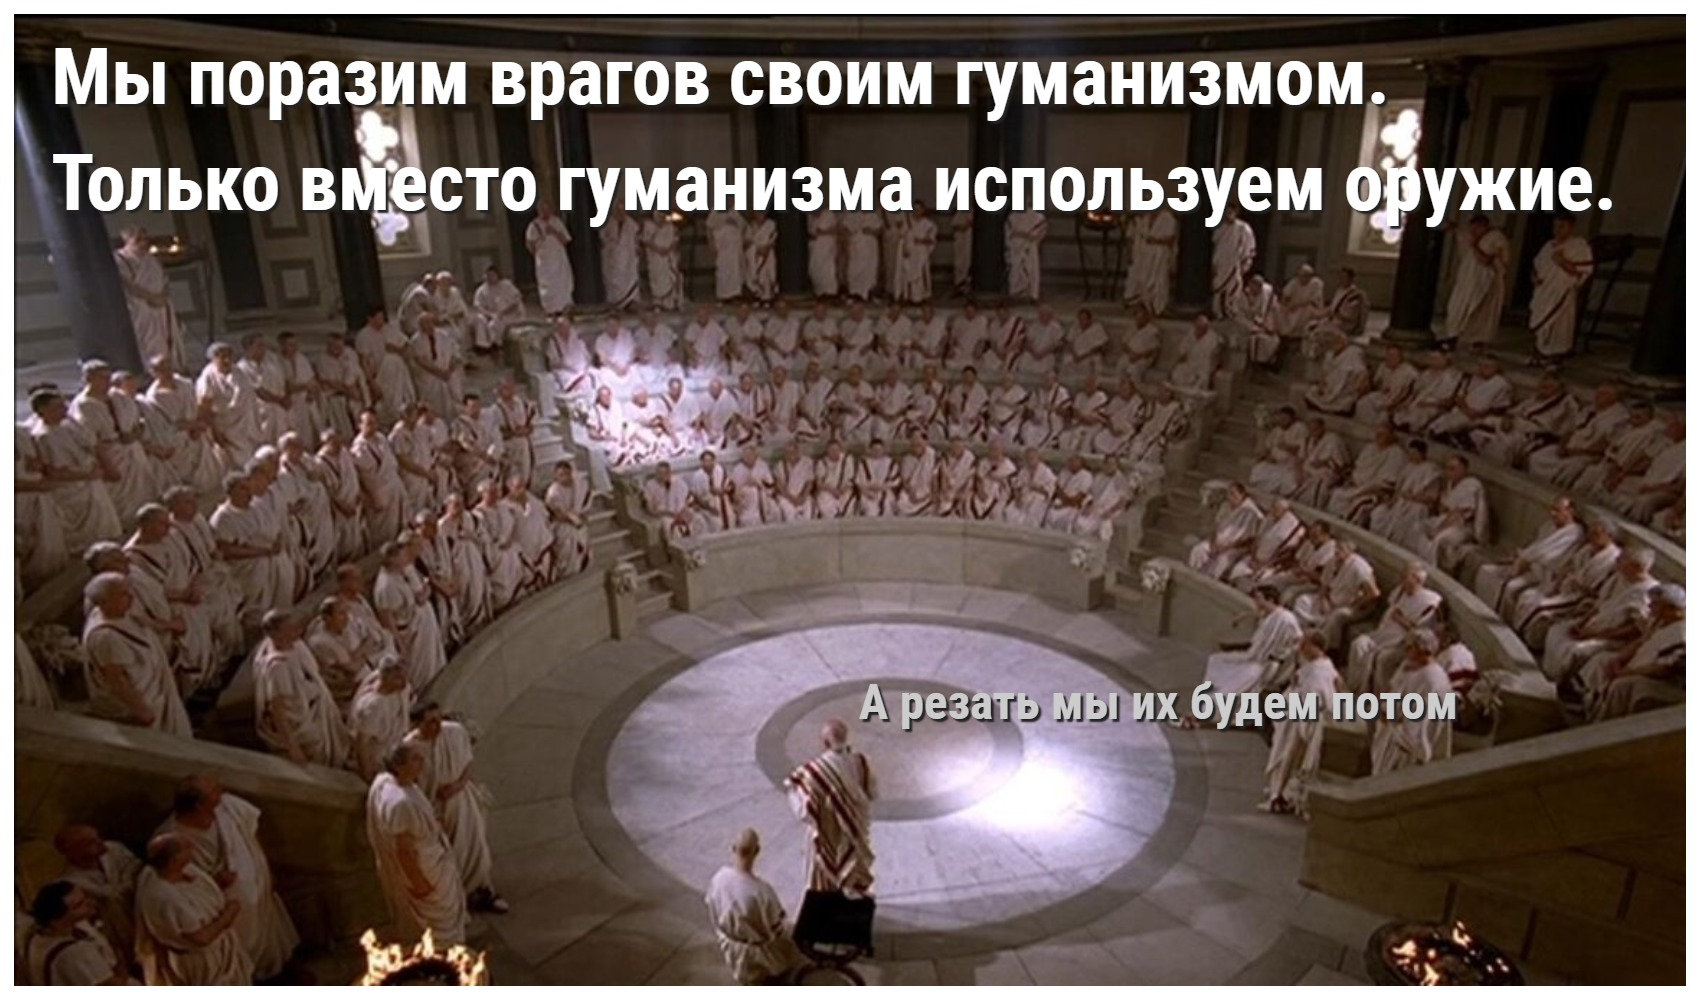
\includegraphics[scale=0.3]{Scipion/1592402098150092058.png}
	%	\label{fig:scipion} % Unique label used for referencing the figure in-text
	%	%\addcontentsline{toc}{figure}{Figure \ref{fig:placeholder}} % Uncomment to add the figure to the table of contents
	%
\end{figure}
